\documentclass[11pt]{book}
\usepackage{amsmath,mathtools}
\usepackage[utf8]{inputenc}
\usepackage[ngerman]{babel}
\usepackage{acronym}
\usepackage{graphicx} 
\usepackage{epstopdf}
\usepackage{svg}
\usepackage{multirow}
\usepackage{amssymb}
\usepackage{trfsigns}
\usepackage{setspace}
\usepackage{yfonts}

\onehalfspacing


%Hyperlinks package, links aus inhaltsverzeichnis
\usepackage{hyperref}
\hypersetup{
    colorlinks=false, %set true if you want colored links
    linktoc=all
}
%Blattformatierung
\usepackage{geometry}
\geometry{a4paper, top=25mm, left=30mm, right=25mm, bottom=20mm}

%Listing
\usepackage{courier}
\usepackage{listings}
\usepackage{color}
 \lstset{
   frame=tb,
   framexleftmargin=2.5em,
   basicstyle=\small\linespread{0.9}\bfseries\ttfamily,
   emph={square}, 
   emphstyle=\color{blue}\texttt,
   emph={[2]root,base},
   emphstyle={[2]\color{yac}\texttt},
   showstringspaces=false,
   flexiblecolumns=false,
   tabsize=2,
   numbers=left,
   numberstyle=\small\bfseries\ttfamily,
   numberblanklines=false,
   stepnumber=1,
   numbersep=10pt,
   xleftmargin=25pt
 }
\begin{document}

\def\presuper#1#2%
	{\mathop{}%
	\mathopen{\vphantom{#2}}^{#1}%
	\kern-\scriptspace%
	#2}
%Display vecotr in a reference frame
\newcommand{\vecBS}[4]{\presuper{#1}{\begin{pmatrix}
#2 \\ #3 \\ #4
\end{pmatrix}}}
%Boldsymbol shortcut
\newcommand{\bs}[1]{\boldsymbol{#1}}
%Bezugssystemdefinition
\newcommand{\defBS}[1]{\{#1\} [ \bs{e}_{{#1}_1},\bs{e}_{{#1}_2}, \bs{e}_{{#1}_3} ]}
%Projektionsmatrix
\newcommand{\pMat}[2]{\presuper{#1}{\bs{P}}^{#2}}
%Differenation in Respekt zu BS
\newcommand{\diffIn}[3]{\frac{\presuper{#1}{d{#2}}}{d#3}}
\newcommand{\partialDiffIn}[3]{\frac{\presuper{#1}{\partial{#2}}}{\partial #3}}
%Geschwindigkeit/Beschleunigung
\newcommand{\vel}[3]{\presuper{#1}{\bs{#2}}^{#3}}

%Rightarrow with spaceing
\newcommand{\rArrow}{\hspace{5pt}\rightarrow\hspace{5pt}}
%Inneres Produkt
\newcommand{\inProd}[2]{\langle {#1}, {#2} \rangle}

%System macro
\newcommand{\cSS}[3]{\textfrak{S}($\bs{#1}$,$\bs{#2}$,$\bs{#3}$)}
\newcommand{\dSS}[3]{\textfrak{D}($\bs{#1}$,$\bs{#2}$,$\bs{#3}$)}

%Laplace transform sign with spaces
\newcommand{\myLaplace}{\hspace{15pt}\laplace\hspace{15pt}}

\newcommand*{\signed}[1]{%
        \nolinebreak[3]\hspace*{\fill}\mbox{\emph{#1}}
    }

\chapter{Regelungstechnik}
Nachdem die Systemdynamik mit Hilfe von Bewegungsgleichungen beschrieben wurde, besteht der nächste Schritt darin ein Regler zu entwerfen, welcher die Stabilisierung des Würfels auf einer Kante ermöglicht. Hierfür wird in diesem Abschnitt zunächst die Beschreibung eines Systems mit Hilfe der Zustandsraumdarstellung diskutiert. Anschließend der Zusammenhang zeitkontinuierlicher Systeme und deren zeitdiskreten Darstellungen ermittelt um den Entwurf von digitalen Reglern zu ermöglichen. Daraufhin werden die Vorteile von Zustandsregler gegenüber klassischen Regelungsalgorithmen verglichen und ein Regler für die Stabilisierung des Würfels auf einer Kante entworfen. Anschließend wird diese Regelungsvorschrift an der reellen Regelstrecke erprobt und validiert. Im letzten Teil werden Beobachter eingesetzt um die Auswirkungen von Messabweichungen zu kompensieren und die Anzahl der nötigen Sensoren zu reduzieren.

\subsection{Beschreibung von System mit Hilfe der Zustandsraumdarstellung}
Aus dem vorherigen Kapitel sind die beiden Bewegungsgleichungen 
\begin{equation}
I_K \cdot \dot{u}_K = m\cdot g\cdot l\cdot s_{\varphi} - C_{\psi}\cdot u_{K} + C_{\psi} \cdot u_{R} - T_M
\end{equation}
\begin{equation}
I_R\cdot \dot{u}_R = C_{\psi}\cdot u_{K} - C_{\psi}\cdot u_{R} + T_M
\end{equation}
hervorgegangen, welche die Systemdynamik vollständig beschreiben. Mit Hilfe der Definitionen
\begin{equation}
\bs{x} = \begin{bmatrix} \varphi \\ u_K \\ u_R \end{bmatrix}
\hspace{35pt}
\bs{y} = \begin{bmatrix} \varphi \\ u_K \\ u_R \end{bmatrix}
\hspace{35pt}
u = T_M
\end{equation}
können die linearisierten Bewegungsgleichungen in die folgende Zustandsraumdarstellung überführt werden.
\begin{equation}
\bs{\dot{x}} = \underbrace{\begin{bmatrix}
0 && 1 && 0 
\\ 
\frac{m\cdot g\cdot l}{I_K} && \frac{-C_{\psi}}{I_K} && \frac{C_{\psi}}{I_K}
\\
0 && \frac{C_{\psi}}{I_R} && \frac{-C_{\psi}}{I_R}
\end{bmatrix}}_{\equiv \bs{A}} \cdot \bs{x}
+
\underbrace{\begin{bmatrix}
0 \\ \frac{-1}{I_K} \\ \frac{1}{I_R}
\end{bmatrix}}_{\equiv \bs{b}} \cdot \bs{u}
\end{equation}
\begin{equation}
\bs{y} = \underbrace{\begin{bmatrix}
1 && 0 && 0 \\ 0 && 1 && 0 \\ 0 && 0 && 1
\end{bmatrix}}_{\equiv \bs{C}} \cdot \bs{x}
\end{equation}
Prinzipiell kann jedes lineare zeitinvariante System %\textfrak{S}
($\bs{A}$, $\bs{B}$, $\bs{C}$, $\bs{D}$) als Zustandsraumdarstellung beschreiben lassen, wobei folgendes gilt.
\begin{equation}
%\textfrak{S} 
: \left\{ \begin{array}{ll}
\bs{\dot{x}}(t) = \bs{A}\cdot \bs{x}(t) + \bs{B}\cdot \bs{u}(t) \\
\bs{y}(t) = \bs{C}\cdot \bs{x}(t) + \bs{D}\cdot \bs{u}(t)
\end{array}
\right.
\end{equation}
Wobei $\bs{x} \in \mathbb{R}^n$ Zustandsvektor, $\bs{u} \in \mathbb{R}^r$ Eingangsvektor und $\bs{y} \in \mathbb{R}^m$ Ausgangsvektor heißt. Im weiteren Verlauf wird die Zeitabhängigkeit dieser drei Vektoren nicht mehr explizit angegeben. Des weiteren werden in dieser Arbeit lediglich nicht sprungfähige Systeme \cSS{A}{B}{C} betrachtet, deren Eingangsvektor $\bs{u}$  den Ausgangsvektor $\bs{y}$ nicht direkt beeinflusst und somit $\bs{D} = \bs{0}$ gilt.

Ein großer Vorteil dieser Modellierungsform besteht darin, dass für jedes Systems unendlich viele Zustandsraumdarstellungen existieren. Dieser Umstand wird ersichtlich wenn man für die Herleitung der Bewegungsgleichungen alternative generalisierte Geschwindigkeiten wählt und diese anschließend in eine Zustandsraumdarstellung transformiert.
\begin{equation}
\tilde{u}_K \equiv \dot{\phi} \hspace{35pt} \tilde{u}_R \equiv \dot{\psi}
\end{equation}
\begin{equation}
I_K\cdot \dot{\tilde{u}}_K = m\cdot g \cdot l \cdot sin_{\varphi} + C_{\psi}\cdot \tilde{u}_R - T_M
\end{equation}
\begin{equation}
I_R\cdot \dot{\tilde{u}}_R = -\frac{I_R\cdot m\cdot g\cdot l\cdot sin_{\varphi}}{I_K} - \frac{(I_K + I_R)\cdot C_{\psi}}{I_K} + \frac{I_K + I_R}{I_K}\cdot T_M
\end{equation}
\begin{equation}
\bs{\dot{\tilde{x}}} = \begin{bmatrix}
0 && 1 && 0 
\\
\frac{m\cdot g\cdot l}{I_K} && 0 && \frac{C_{\psi}}{I_K}
\\
\frac{-I_R\cdot m\cdot g\cdot l}{I_R\cdot I_K} && 0 && \frac{-C_{\psi}(I_K+I_R)}{I_R\cdot I_K} 
\end{bmatrix}\cdot \bs{\tilde{x}}
+
\begin{bmatrix}
0 \\ \frac{-1}{I_K} \\ \frac{I_K+I_R}{I_K\cdot I_R}
\end{bmatrix} \cdot u
\end{equation}
\begin{equation}
\bs{y} = \begin{bmatrix}
1 && 0 && 0 \\
0 && 1 && 0 \\
0 && 1 && 1 \\
\end{bmatrix} \cdot \bs{\tilde{x}}
\end{equation}

Sowohl die verschiedenen Bewegungsgleichungen als auch die daraus resultierenden Zustandsraumdarstellungen sind gültige Beschreibungsformen des Systems. Allgemein kann ein Zustandsraumdarstellung mit Hilfe einer Transformationsmatrix $\bs{T} \in \mathbb{R}^{n\times n}$ in eine äquivalente Darstellung überführt werden. Hierfür muss $\bs{T}$ lediglich regulär sein. Die neue Darstellung ergibt sich aus den folgenden Transformationen.
\begin{equation}
\bs{\tilde{x}} = \bs{T}^{-1}\cdot\bs{x} \hspace{35pt}\bs{\dot{\tilde{x}}} = \bs{T}^{-1}\cdot \bs{\dot{x}}
\end{equation}
\begin{equation}
\begin{split}
\bs{\dot{\tilde{x}}} &= \bs{T}^{-1}\bs{A}\bs{T}\cdot \bs{\tilde{x}} + \bs{T}^{-1}\cdot \bs{u} \\
& = \bs{\tilde{A}}\cdot \bs{\tilde{x}} + \bs{\tilde{B}}\cdot \bs{u} \hspace{45pt} \vert \hspace{15pt} \bs{\tilde{A}} = \bs{T}^{-1}\bs{A}\bs{T}, \bs{\tilde{B}} = \bs{T}^{-1}\bs{B}
\end{split}
\end{equation}
\begin{equation}
\bs{y} = \bs{C}\bs{T}\cdot \bs{\tilde{x}} 
= \bs{\tilde{C}}\cdot \bs{\tilde{x}} \hspace{45pt} \vert \hspace{15pt} \bs{\tilde{C}} = \bs{C}\bs{T}
\end{equation}
Mit Hilfe derartiger Transformationen kann ein beliebiges System in diverse Normalformen überführt werden, welche für die Systemanalyse und den Reglerentwurf besonders geeignet sind. Als erstes Beispiel sei die Transformation in kanonische Normalform genannt. Hierfür sei ein System \cSS{A}{B}{C} der Ordnung $n$ gegeben, dessen Systemmatrix $\bs{A}$ $n$ einfache Eigenwerte $\lambda_i$ mit den zugehörigen Eigenvektoren $\bs{v}_i$ besitzt. Sind die Eigenvektoren $\bs{v}_i$ linear unabhängig dann ist die Matrix
\begin{equation}
\bs{V} = \begin{bmatrix}
\bs{v}_i & \bs{v}_2 & \hdots & \bs{v}_n 
\end{bmatrix}
\end{equation}
regulär und kann somit als Transformationsmatrix verwendet werden. Die resultierende Darstellung
\begin{equation}
\begin{split}
\bs{\dot{\tilde{x}}} &= \bs{V}^{-1}\bs{A}\bs{V}\cdot \bs{\tilde{x}} + \bs{V}^{-1}\bs{B}\cdot \bs{u} \\
\bs{y} &= \bs{C}\bs{V}\cdot \bs{\tilde{x}}
\end{split}
\end{equation}
heißt kanonische Normalform, wobei die Matrix $\bs{\tilde{A}}$ die folgende Form besitzt.
\begin{equation}
\bs{\tilde{A}} = \bs{V}^{-1}\bs{A}\bs{V} = \begin{bmatrix}
\lambda_1 & 0 & \hdots & 0 \\
0 & \lambda_2 & \hdots & 0 \\
\vdots & \vdots & \ddots & \vdots \\
0 & 0 & \hdots & \lambda_n
\end{bmatrix}
\end{equation}
Folglich sind die Elemente des Zustandvektors $\bs{\tilde{x}}$ vollständig voneinander entkoppelt und werden deshalb auch als Eigenvorgänge bzw. Eigenbewegungen des Systems bezeichnet. Die vollständige Entkopplung der Zustandsgrößen ist nicht immer mögliche, für eine ausführliche Diskussion Thematik sei auf [RT1, Lunze, S.135ff] verwiesen.
Die homogenen Lösung der kanonischen Normalform lässt sich mit Hilfe des Exponentialansatzes ermitteln.
\begin{equation}
\tilde{x}_{i,h}(t) = e^{\lambda_i\cdot t}\cdot \tilde{x}_i(0) \rArrow \bs{\tilde{x}}_h(t) = \begin{bmatrix}
e^{\lambda_1\cdot t} &  & \\
& e^{\lambda_2\cdot t}  & \\
&  & \ddots & \\
&  & & e^{\lambda_n\cdot t}
\end{bmatrix}\cdot \bs{\tilde{x}}(0)
\end{equation}
Die Rücktransformation
\begin{equation}
\bs{x}_h = \bs{V}\cdot \bs{\tilde{x}}_h
\end{equation}
zeigt, dass der Verlauf der ursprünglichen Zustandsgrößen eine Linearkombination der kanonischen Zustandsvariablen ist. Folglich wird die homogenen Lösung eines Systems durch die Eigenwerte und -vektoren der Systemmatrix $\bs{A}$ vorgegeben. 
Formal kann dieser Zusammenhang durch die Erweiterung des Exponentialansatzes auf vektorwertige Differentialgleichungen ermittelt werden.
\begin{equation}
\bs{x}(t) = e^{\bs{A}\cdot t}\cdot \bs{x}(0) + \int^t_0 e^{\bs{A}(t-\tau)}\bs{B}\cdot \bs{u}(\tau)d\tau
\label{eq_fMat_zeitbereich}
\end{equation}
Die Matrix-Exponentialfunktion $e^{\bs{A}\cdot t}$ heißt Fundamentalmatrix $\bs{\Phi}(t)$ und kann über die folgende Reihenentwicklung bestimmt werden. Eine Herleitung kann in [RT2, Unbehauen, S. 6. ff] gefunden werden. 
\begin{equation}
\bs{\Phi}(t) = e^{\bs{A}\cdot t} = \sum^{\infty}_{k=0} \bs{A}^k\frac{t^k}{k!}
\end{equation}
Um einen weiteren Weg zur Ermittlung der Fundamentalmatrix und den Zusammenhang zu der Übertragungsfunktion des Systems herzustellen wird die Systemgleichung in den Bildbereich transformiert.
\begin{equation}
\begin{split}
\bs{\dot{x}}(t) = \bs{A}\cdot \bs{x}(t) + \bs{B}\cdot\bs{u}(t) \myLaplace &s\cdot\bs{x}(s) - \bs{x}(t=0) = \bs{A}\cdot \bs{x}(s) + \bs{B}\cdot \bs{u}
\\
\leftrightarrow \hspace{15pt} &\bs{x}(s) = \underbrace{(s\cdot \bs{I} - \bs{A})^{-1}}_{\equiv \bs{\Phi}(s)}\bs{x}(t=0) + (s\cdot \bs{I}-\bs{A})^{-1}\bs{B}\cdot \bs{u}(s) 
\\
\leftrightarrow \hspace{15pt}&\bs{x}(s) = \bs{\Phi}(s)\cdot \bs{x}(t=0) +\bs{\Phi}(s)\bs{B}\cdot \bs{u}(s)
\end{split}
\label{eq_fMat_bildbereich}
\end{equation}
Aus dem Vergleich von (\cite{eq_fMat_bildbereich}) mit (\cite{eq_fMat_zeitbereich}) wird ersichtlich, dass die Fundamentalmatrix im Bildbereich durch die Invertierung der Matrix $s\cdot \bs{I}-\bs{A}$ berechnet werden kann. Im nächsten Schritt wird lediglich das Übertragungsverhalten eines Systems betrachtet.
\begin{equation}
\bs{x}(s) = \bs{\Phi}(s)\bs{B}\cdot \bs{u}(s) \hspace{35pt} \vert \hspace{15pt} \bs{x}(t=0) = 0
\end{equation}
\begin{equation}
\bs{y}(s) = \bs{C}\cdot \bs{x}(s) = \underbrace{\bs{C}\bs{\Phi}(s)\bs{B}}_{\equiv \bs{G}(s)}\cdot \bs{u}(s) = \bs{G}(s)\cdot \bs{u}(s)
\end{equation}
Im Falle eines SISO-Systems reduzieren sich die Matrizen $\bs{C}$ und $\bs{B}$ auf die Vektoren $\bs{c^T}$ und $\bs{b}$. Somit handelt es sich bei $G(s)$ um die Übertragungsfunktion des Eingrößensystems. Bei MIMO-Systemen heißt $\bs{G}(s)$ Übertragungsfunktionmatrix, wobei die einzelnen Elemente $G_{ij}(s)$ Teilübertragungsfunktionen heißen und das E/A-Verhalten der Eingangsgröße $u_j$ auf die Ausgangsgröße $y_i$ beschreiben. Bei der Berechnung der Übertragungsmatrix $\bs{G}(s)$ stellt die Fundamentalmatrix $\bs{\Phi}(s)$ die einzige Größe dar, die von $s$ abhängt, und muss somit auch die Pole des Systems enthalten. Aus der Berechnung
\begin{equation}
\bs{\Phi}(s) = (s\cdot \bs{I}-\bs{A})^{-1} = \frac{1}{det(s\cdot \bs{I}  - \bs{A}}adj(s\cdot \bs{I} - \bs{A})
\end{equation}
folgt, dass das charakteristische Polynom
\begin{equation}
det(s\cdot \bs{I}-\bs{A})
\end{equation}
den gemeinsamen Nenner der Teilübertragungsfunktionen darstellt. Die Nullstellen des Polynoms entsprechen den Eigenwerten der Systemmatrix $\bs{A}$. Hieraus folgt, dass die Eigenwerte $\lambda_i$ eine Übermenge der Pole $s_i$ des Systems bilden, da ggf. Eigenwerte gegen  Zählernullstellen gekürzt werden können.
Dies bedeutet, dass die Systemmatrix $\bs{A}$ nicht nur die Eigenbewegung des Systems bestimmt sondern auch zur Untersuchung der Stabilität verwendet werden kann. Allgemein ist ein System asymptotisch stabil wenn die Realteile aller Eigenwerte $\lambda_i$ der Matrix $\bs{A}$ negativ sind.
\begin{equation}
Re{\lambda_i} < 0
\end{equation}
Dieses Stabilitätskriterium stellt einen weiteren Vorteil der Systembeschreibung mittels Zustandsraumdarstellung dar. Die Systemanalyse erfolgt durch die Unterschung numerischer Matrizen, was mit Hilfe von Matlab effizient umgesetzt werden kann. Des weiteren müssen bei MIMO-Systemen mit klassischen Stabilitätskriterien alle Elemente der Übertragungsfunktionsmatrix $\bs{G}(s)$ untersucht werden. In der Zustandsraumdarstellung genügt allerdings die Analyse der Systemmatrix $\bs{A}$.


\section{Zustandsraumdarstellung für zeitdiskrete Systeme}
Bisher wurden ausschließlich zeitkontinuierliche Systeme betrachtet. Allerdings wird der Regler mit Hilfe eines Digitalrechners implementiert und stellt somit ein zeitdiskretes Systems dar. Derartige Systeme werden in Form von Differenzengleichungen beschrieben, die ebenfalls in eine Zustandsraumdarstellung überführt werden können. Hierbei wird lediglich der Integrierer durch ein vektorielles Totzeitglied ersetzt, welches eine Abtastperiode darstellt. Somit gilt für ein diskretes System 
\begin{equation}
\textfrak{D} : \left\{ \begin{array}{ll}
\bs{{x}}(k+1) = \bs{A_d}\cdot \bs{x}(k) + \bs{B_d}\cdot \bs{u}(k) \\
\bs{y}(k) = \bs{C_d}\cdot \bs{x}(k)
\end{array}
\right.
\label{eq_discrete_ss}
\end{equation}
Die Ergebnisse aus dem vorherigen Abschnitt können auf diskrete Systeme übertragen werden. Hierfür wird zunächst die Z-Transformierte der Systemgleichung betrachtet.
\begin{align}
\bs{x}(k+1) &= \bs{A}\cdot \bs{x}(k)+\bs{B}\cdot \bs{u}(k)
\nonumber
\\ \myLaplace  &z\cdot \left[\bs{x}(z)- \bs{x}(t=0)\right] = \bs{A_d}\cdot \bs{x}(z) + \bs{B_d}\cdot \bs{u}(z) \nonumber
\\
\hspace{15pt}\leftrightarrow\hspace{20pt}
&(z\cdot\bs{I}-\bs{A_d})\bs{x}(z) = z\cdot \bs{x}(t=0)+\bs{B_d}\cdot \bs{u}(z) \nonumber
\\
\hspace{15pt}\leftrightarrow\hspace{20pt}
&\bs{x}(z) = \underbrace{(z\cdot\bs{I}-\bs{A_d})^{-1}}_{\equiv \bs{\Phi_d}(z)}\cdot z\cdot \bs{x}(t=0) + (z\cdot \bs{I}-\bs{A_d})^{-1}\bs{B_d}\cdot \bs{u}(z)
\end{align}
\begin{equation}
\bs{y}(z) = \bs{C_d}\cdot \bs{x}(z) = \underbrace{\bs{C_d}\bs{\Phi_d}(z)\bs{B_d}}_{\equiv \bs{G_d}(z)}\cdot \bs{u}(z)
\end{equation}
An Hand der obigen Gleichungen ist leicht zu erkennen, dass sowohl die Fundamentalmatrix $\bs{\Phi_d}(z)$ als auch die Übertragungsfunktionmatrix $\bs{G_d}(z)$ analog zu zeitkontinuierlichen Systemen berechnet wird. Deshalb behalten die Eigenwerte und -vektoren der Systemmatrix $\bs{A_d}$ ihre Bedeutung für die Systemenanalyse. Lediglich die Interpretation muss durch den Zusammenhang der Laplace- und Z-Transformation angepasst werden.
\begin{equation}
z = e^{T\cdot s} \hspace{35pt} s = \sigma + j\cdot \omega
\end{equation}
\begin{equation}
\vert z \vert = e^{T\cdot \sigma} \hspace{35pt} \phi = \omega\cdot T
\label{eq_abs_z}
\end{equation}
Stabilitätsbedingung für kontinuierliche Systeme ist, dass die Realteile aller Eigenwerte $\lambda_i$ negativ sind. Aus (\ref{eq_abs_z}) folgt, dass der Betrag der diskreten Eigenwerte im Einheitskreis liegen muss, damit diese Forderung erfüllt ist. Des weiteren führen diskrete Eigenwerte, die nahe am Ursprung liegen, zu einer schnelleren Systemdynamik. Somit bringt Zustandsraumdarstellung für diskrete Systeme die gleichen Vorteile mit sich wie bei zeitkontinuierlichen Systemen.
Allerdings handelt es sich bei der Regelstrecke nach wie vor um ein kontinuerliches System, lediglich der Regler stellt ein diskretes System dar. Die Schnittstelle zwischen der kontinuierlichen Strecke und dem diskreten Regler ist einerseits ein Abtastglied, welches den Zustandsvektors $\bs{x}(t)$ in die Zahlenfolge $\bs{x}(k)$ überführt. Andererseits wird die Folge der Stellgröße $\bs{u}(k)$ mit Hilfe eines Halteglieds nullter Ordnung als eine kontinuierliche Treppenfunktion moduliert.

Um den geschlossenen Regelkreis einheitlich zu beschreiben, muss deshalb die kontinuierliche Zustandsarumdarstellung der Regelstrecke in eine diskrete transformiert werden. Hierzu wird zunächst die Lösung eines kontinuierlichen Systems \cSS{A}{B}{C} betrachtet.\footnote{Die folgende Herleitung und Erklärung ist nach ([RT2, Unbehauen, S. 170 f.) paraphrasiert.} Herleitung aus [RT2, Unbehauen]
\begin{equation}
\bs{x}(t) = e^{\bs{A}\cdot t}\cdot \bs{x}(t_0) + \int^t_0 e^{\bs{A}(t-\tau)}\bs{B}\cdot \bs{u}(\tau)d\tau
\end{equation}
Der Verlauf zwischen zwei Abtastzeitpunkten $(k+1)T$ und $kT$ wird berechnet indem $t_0=kT$ und $t=(k+1)T$ gilt.
\begin{equation}
\begin{split}
\bs{x}( (k+1)T) &= e^{\bs{A}(k+1)T}\cdot \bs{x}(kT) + \int^{(k+1)T}_{kT} e^{\bs{A}([k+1]T-\tau}\bs{B}\bs{u}(\tau)d\tau \\
&= e^{\bs{A}(k+1)T}\cdot \bs{x}(kT) + \int^T_0 e^{\bs{A}(kT-\tau)}\bs{B}\bs{u}(\tau)d\tau
\end{split}
\end{equation}
Um das Integral zu lösen muss der Verlauf von $\bs{u}$ zwischen den Abtastpunkten bekannt sein. Das Halteglied nullter Ordnung führt die diskrete Zahlenfolge der Stellgröße $\bs{u}(k)$ in eine kontinuierliche Treppenfunktion über. Somit folgt, dass $\bs{u}$ über den Verlauf einer Abtastperiode konstant ist.
\begin{equation}
\bs{u}(kT+t) = \bs{u}(kT) \hspace{35pt} \vert \hspace{15pt} 0 \leqslant t < T
\end{equation}
Die Lösung des Integrals führt auf:
\begin{equation}
\bs{x}([k+1]T) = e^{\bs{A}T}\cdot \bs{x}(kT) + e^{\bs{A}T}(\bs{I}-e^{-\bs{A}T})\bs{A}^{-1}\bs{B}\cdot \bs{u}(kT)
\end{equation}
Diese Lösung stellt den Zusammenhang zwischen der kontinuierlichen und diskreten Zustandsraumdarstellung dar. Wobei der Vergleich mit (\ref{eq_discrete_ss}) folgenden Werte für die Matrizen des diskreten Systems \dSS{A_d}{B_d}{C_d} liefert.
\begin{equation}
\bs{A_d} = e^{\bs{A}T} \hspace{35pt} \bs{B_d} = (e^{\bs{A}T}-\bs{I})\bs{A}^{-1}\bs{B} \hspace{35pt} \bs{C_d} = \bs{C}
\end{equation}
Mit der Definition
\begin{equation}
\bs{S} = T \sum^{\infty}_{v=0}\bs{A}^v\frac{T^v}{(v+1)!}
\end{equation}
kann die Definition vereinfacht und die Berechnung der inversen Matrix vermieden werden.
\begin{equation}
\bs{A_d} = \bs{I}+\bs{S}\bs{A}\hspace{35pt} \bs{B_d} = \bs{SB}
\end{equation}
Die Matrix $\bs{S}$ beschreibt einerseits den Einfluss des Halteglieds auf den Regelkreis, andererseits ermöglicht sie die Überführung in eine diskrete Darstellung, welche nötig ist um die Regelstrecke und den Regler in einer einheitlichen Form zu beschreiben. 

\section{Entwurf von Zustandsregelungen}
Nachdem die Grundlagen der Zustandsraumdarstellung in den vorherigen Abschnitten diskutiert wurden, dient dieser Teil dem Entwurf des letztendlichen Reglers. Hierfür wird zunächst am Beispiel des Entwurfs durch Eigenwertvorgabe der Grundgedanke und die Vorteile der Zustandsregelung aufgezeigt. Anschließend wird ein Regler nach dem Prinzip der optimalen Regelung entworfen um den Würfel auf einer Kante zu stabilisieren. Diese Ergebnisse werden an der reellen Regelstrecke überprüft.

\subsection{Reglerentwurf durch Eigenwertvorgabe}
Der Grundgedanke der Zustandsregelung besteht darin den vollständigen Zustandsvektor $\bs{x}$ zurückzuführen und durch die Multiplikation mit einer Reglermatrix $\bs{K}$ den Stellgrößenvektor $\bs{u}$ zu ermitteln. In dieser Arbeit werden lediglich Regelkreise ohne Führungsvektor ($\bs{w}=\bs{0})$) verwendet, weshalb auf dessen Einfluss und den Entwurf des nötigen Vorfilters $\bs{V}$ nicht weiter eingegangen wird.
\begin{figure}[H]
\centering
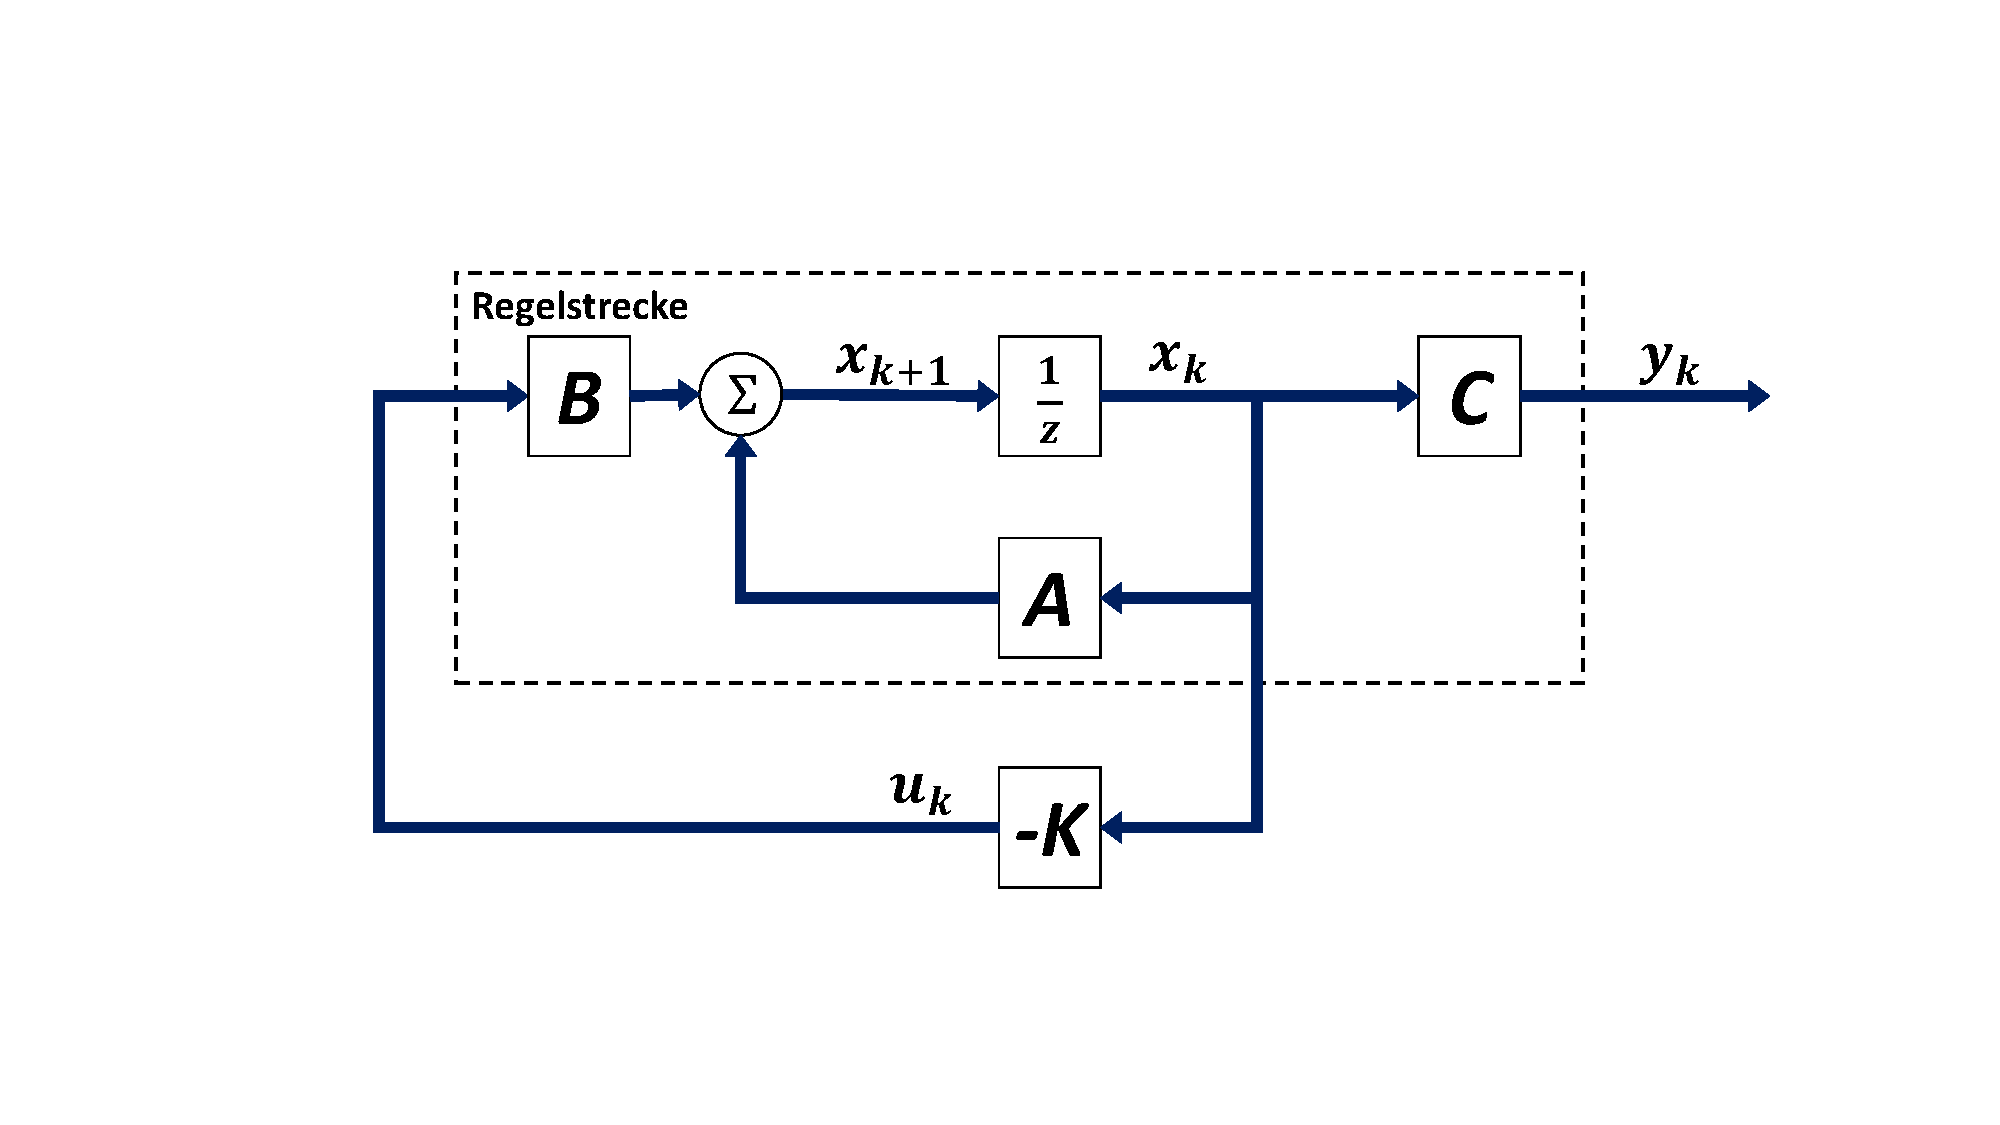
\includegraphics[width=0.8\linewidth, trim={3.5cm 3.5cm 3.5cm 3.5cm}, clip]{img/RT_ClosedLoop}
\caption{Signalfluss des geschlossenen Regelkreises, Quelle: eigene Darstellung}
\end{figure}
Aus der Abbildung gehen die Systemgleichungen des geschlossenen Regelkreises $\overline{\textfrak{D}}$($\overline{\bs{A}}$,$\bs{0}$, $\overline{\bs{C}}$) hervor.
\begin{equation}
\bs{u}(k) = -\bs{B}\bs{K}\cdot\bs{x}(k)
\end{equation}
\begin{equation}
\overline{\textfrak{D}}
: \left\{ \begin{array}{ll}
\bs{{x}}(k+1) &= \bs{A}\cdot \bs{x}(k) - \bs{B}\bs{K}\cdot \bs{x}(k) = \underbrace{(\bs{A}-\bs{B}\bs{K})}_{\equiv \bs{\overline{A}}}\cdot \bs{x}(k) \\
\bs{y}(k) &= \underbrace{\bs{C}}_{\equiv \bs{\overline{C}}}\cdot \bs{x}(k)
\end{array}
\right.
\end{equation}
Die Reglermatrix $\bs{K}$ ist nun so zu entwerfen, dass die gewünschten Eigenschaften des geschlossenen Regelkreises erreicht werden. Hierfür wird zunächst das SISO-System \dSS{A}{b}{c^T} betrachtet, wessen Systemmatrix $\bs{A}$ und Eingangsvektor $\bs{b}$ die folgende Form besitzt.
\begin{equation}
\bs{A} = \begin{bmatrix}
0 & 1 & 0 & \hdots & 0 \\
0 & 0 & 1 & \hdots & 0 \\
\vdots & \vdots & \vdots & \ddots & \vdots \\
-a\idx0 & -a\idx1 & -a\idx2 & \hdots & -a_{n-1}
\end{bmatrix}
\hspace{35pt}
\bs{b} = \begin{bmatrix}
0 \\ 0 \\ \vdots \\ 1
\end{bmatrix}
\end{equation}
Diese Darstellung heißt Regelungsnormalform und kann mittels einer Zustandstransformation erreicht werden. Diese Transformation wird hier nicht näher erläutert, da das Verfahren lediglich als Beispiel der Zustandsregelung dienen soll.\footnote{Die Bestimmung der Transformationsmatrix und der Erweiterung des Entwurfsverfahren durch Eigenwertvorgabe kann in (RT2, Lunze, S. 245) nachgelesen werden.} Der besondere Vorteil der Regelungsnormalform besteht darin, dass die Werte $a_i$ die Koeffizienten des charakteristischen Polynoms 
\begin{equation}
\text{det}(\lambda\cdot \bs{I}-\bs{A}) = \prod^n_{i=1} (\lambda-\lambda_i) = \lambda^n+a_{n-1}\cdot \lambda^{n-1} + \hdots + a\idx1\cdot \lambda + a\idx0
\end{equation}
der Systemmatrix $\bs{A}$ sind. Wird der Regelkreis über den Reglervektor
\begin{equation}
\bs{k} = \begin{bmatrix}
k_1 & k_2 & \hdots & k_n
\end{bmatrix}
\end{equation}
geschlossen, ergibt sich sich die  Systemmatrix $\bs{\overline{A}}$ des geschlossenen Regelkreises
\begin{equation}
\begin{split}
\bs{\overline{A}} = \bs{A}-\bs{b}\bs{k} &= \begin{bmatrix}
0 & 1 & 0 & \hdots & 0 \\
0 & 0 & 1 & \hdots & 0 \\
\vdots & \vdots & \vdots & \ddots & \vdots \\
-a\idx0 & -a\idx1 & -a\idx2 & \hdots & -a_{n-1}
\end{bmatrix}
-
\begin{bmatrix}
0 & 0 & 0 & \hdots & 0 \\
0 & 0 & 0 & \hdots & 0 \\
\vdots & \vdots & \vdots &  \ddots & \vdots \\
k\idx1 & k\idx2 & k\idx3 & \hdots & k_n
\end{bmatrix}
\\
&= \begin{bmatrix}
0 & 1 & 0 & \hdots & 0 \\
0 & 0 & 1 & \hdots & 0 \\
\vdots & \vdots & \vdots & \ddots & \vdots \\
-\overline{a}\idx0 & -\overline{a}\idx1 & -\overline{a}\idx2 & \hdots & -\overline{a}_{n-1}
\end{bmatrix}
\hspace{25pt} \vert \hspace{15pt} \overline{a}_i = a_i + k_{i+1} \,.
\end{split}
\end{equation}
Die Systemmatrix $\bs{\overline{A}}$ des geschlossenen Regelkreises liegt nun ebenfalls in Regelungsnormalform vor, weshalb wiederum für deren charakteristisches Polynom
\begin{equation}
\text{det}(\lambda\cdot \bs{I}-\bs{\overline{A}}) = \prod^n_{i=1} (\lambda-\overline{\lambda}_i) = \lambda^n+\overline{a}_{n-1}\cdot \lambda^{n-1} + \hdots + \overline{a}\idx1\cdot \lambda + \overline{a}\idx0
\label{eq_ew_gRK}
\end{equation}
gilt. Werden nun die Eigenwerte $\overline{\lambda}_i$ des geschlossenen Regelkreises vorgegeben können durch (\ref{eq_ew_gRK}) die Koeffizienten $\overline{a}_i$ berechnet werden. Die Koeffizienten $a_i$ der Regelstrecke werden aus der Matrix $\bs{A}$ abgelesen werden. Somit können aus der Beziehung
\begin{equation}
\overline{a}_i = a_i + k_i
\end{equation}
die einzelnen Regerfaktoren $k_i$ berechnet werden. Diese führen in dem geschlossenen Regelkreis auf die vorgegebenen Eigenwerte $\overline{\lambda}_i$. Alternativ kann auch die folgende Vektorschreibweise verwendet werden.
\begin{equation}
\underbrace{
\begin{bmatrix}
\overline{a}_0 & \overline{a}_1 & \hdots &\overline{a}_{n-1}
\end{bmatrix}}_{\equiv \bs{\overline{a}}}
=
\underbrace{
\begin{bmatrix}
a_0 & a_1 & \hdots & a_{n-1}
\end{bmatrix}}_{\equiv \bs{a}}
+
\underbrace{
\begin{bmatrix}
k_1 & k_2 & \hdots & k_n
\end{bmatrix}}_{\equiv \bs{k}}
\end{equation}
\begin{equation}
\bs{k} = \bs{\overline{a}} - \bs{a}
\end{equation}
An diesem Entwurfsverfahren werden bereits einige interessante Eigenschaften der Zustandsregelung deutlich. Zunächst können die Eigenwerte des geschlossenen Regelkreises beliebig gewählt werden wodurch das dynamische Verhalten maßgeblich bestimmt wird. Des weiteren wird der Regler durch eine Matrix-Vektor-Multiplikation realisiert. Somit werden dem Regelkreis, im Gegensatz zu PID-Reglern, keine weiteren Pole durch die Reglerdynamik hinzugefügt. Zuletzt sei die einfache Berechnung der Reglermatrix erwähnt. Sowohl die Transformation auf Regelungsnormalform als auch die Ermittlung der Regerparameter sind numerische Operationen die mit Hilfe von Matlab durchgeführt werden können.

Dennoch wird das Entwurfsverfahren in dieser Arbeit nicht verwendet. Die Gründe hierfür sind, dass das primäre Ziel darin besteht eine robuste Regelung zur Stabilisierung des Systems zu entwerfen und nicht eine spezielle Dynamik des geschlossenen Regelkreises zu erzielen. Des weiteren können bei diesem Verfahren die Verläufe der physikalischen Größen $\varphi$, $u_K$ und $u_R$ nicht direkt beeinflusst werden. Durch die Vorgabe der Eigenwerte werden lediglich die Trajektorien der kanonischen Zustandsvariablen bestimmt, welche jeweils eine Linearkombination der ursprünglichen Zustände sind. Des weiteren fließt die Stellgröße $u$ bei dieser Vorgehensweise nicht in die Bestimmung der Reglermatrix ein. Ist die Stellgröße, wie in den hier behandelten Anwendungsfällen, begrenzt müssen diese Umstände bei dem Reglerentwurf beachtet werden.

\subsection{Linear quadratisch optimale Regelung}
Im vorherigen Abschnitt wurden die Nachteile der Eigewertvorgabe aufgezeigt, weshalb hier der Entwurf eines linear quadratisch optimalen Reglers vorgestellt und an der realen Regelstrecke appliziert wird. Der Grundgedanke der optimalen Regelung ist es ein Regelgesetz zu entwerfen, welches zu einem geschlossenen Regelkreis führt, der im Sinne eines Gütekriteriums optimal ist. Hier wird das linear quadratische Gütekriterium
\begin{equation}
J = \sum^{\infty}_{k=0} \left[\bs{x}^T(k)\cdot \bs{Q} \cdot \bs{x}(k) + \bs{u}^T(k)\cdot \bs{R}\cdot \bs{u}(k)\right]
\end{equation}
verwendet. Die Matrizen $\bs{Q}$ und $\bs{R}$ dienen der Gewichtung des Zustands- bzw. Stellvektors und müssen positiv semidefinit bzw. definit sein. Durch die Gewichtungsmatrizen ist es möglich Forderung an den ursprünglichen Zustands- und Stellvektor direkt in den Reglerentwurf einfließen zu lassen. Der letztendliche Regler ergibt sich aus der Lösung des Optimierungsproblems, dass $J$ minimal wird. Nach [Ludyk, S.177] gilt für die Reglermatrix
\begin{equation}
\bs{K} = (\bs{R}+\bs{B}^T\bs{P}\bs{B})^{-1}\bs{B}^T\bs{P}\bs{A}\,,
\end{equation}
wobei $\bs{P}$ durch die Lösung der Matrix-Ricatti-Gleichung 
\begin{equation}
\bs{P} = \bs{Q}+\bs{A}^T[\bs{P}-\bs{P}\bs{B}(\bs{R}+\bs{B}^T\bs{P}\bs{B})^{-1}\bs{B}^T\bs{P}]\bs{A}
\end{equation}
bestimmt wird. Ähnlich wie bei dem Entwurf durch Eigenwertvorgabe besteht ein Vorteil der linear quadratisch optimalen Regelung darin, dass das Optimierungsproblem mittels des Matlab-Befehls \textit{dlqr()} gelöst werden kann. Somit fällt der Rechenaufwand für die Ermittlung der Reglermatrix bei der Bewertung des Entwurfverfahrens nicht weiter ins Gewicht. Deshalb werden hier lediglich die Bedeutung der Gewichtsmatrizen und die Eigenschaften des resultierenden Regelkreises diskutiert.

Hierfür müssen zunächst die Begriffe der Steuerbarkeit und Beobachtbarkeit erklärt werden. Bei einem vollständig steuerbaren System kann, durch eine passende Wahl des Stellvektors $\bs{u}$, der Zustandsvektor $\bs{x}$ in einen beliebigen Wert überführt werden. Zum Beispiel ist ein SISO-System in kanonischer Normalform mit einfachen Eigenwerten steuerbar, wenn alle Elemente $b_{i}$ des Einganvektors $\bs{\tilde{b}}$ ungleich null sind. Ist eines der Elemente $b_{i}$ gleich null kann der zugehörige Zustand $\tilde{x}_i$ nicht durch die Eingangsgröße beeinflusst werden und ist somit nicht steuerbar. Folglich kann auch dieser Eigenwert durch einen Regler nicht beeinflusst werden. Die Definition der Steuerbarkeit lautet:

\begin{quote}
\glqq Ein System $\Sigma$ heißt vollständig steuerbar, wenn es in endlicher Zeit $t_e$ von jedem beliebigen Anfangszustand $\bs{x}_0$ durch eine geeignet gewählte Eingangsgröße $\bs{u}_{[0,t_e]}$ in einen beliebig vorgegebenen Endzustand $\bs{x}(t_e)$ überführt werden kann.\grqq
\signed{LunzeRT2, S. 64}
\end{quote}

Umgekehrt beschreibt die Beobachtbarkeit die Möglichkeit den Zustandsvektor eines Systems aus dem Verlauf des Eingang- und Ausgangvektors zu rekonstruieren.

\begin{quote}
\glqq Ein System $\Sigma = (\bs{A},\bs{B},\bs{C})$ hießt vollständig beobachtbar, wenn der Anfangszustand $\bs{x}_0$ aus dem über einem endlichen Intervall $[0,t_e]$ bekannten Verlauf der Eingangsgröße $\bs{u}_{[0,t_e]}$ und der Ausgangsgröße $\bs{y}_{[0,t_e]}$ bestimmt werden kann.\grqq
\signed{LunzeRT2, S. 92}
\end{quote}

Um sowohl die Steuer- als auch Beobachtbarkeit eines Systems zu prüfen können die Kalmankritieren angewandt werden [LunzeRT2, S.93ff]. Für den Entwurf eines Zustandsregler muss ein System mindestens stabilisierbar sein. Dies bedeutet, dass alle instabilen Eingevorgänge des System sowohl steuer- als auch beobachtbar sind. Für diesen Fall lässt sich zeigen [Lunze RT2, S.301], dass der Entwurf nach dem linear qudratischen Gütekriterium zu einem asymptotisch stabilen Regelkreis führt. Hieraus folgt, dass alle Eigenwerte des geschlossenen Regelkreises im Einheitskreises liegen. Des weiteren lässt sich durch
\begin{equation}
\vert z\vert = e^{\sigma_i} \hspace{35pt} \vert \hspace{15pt} s_i = \sigma_i + \omega_i\cdot j
\end{equation}
der Abstand der Eigenwerte zum Ursprung der komplexen Ebene interpretieren. Je näher ein Eigenwert am Ursprung liegt, desto schneller wird die zugehörige Eigenbewegung. Im geschlossenen Regelkreis wird eine schnelle Systemdynamik durch hohe Stellgrößen verursacht, welche durch die Reglermatrix $\bs{K}$ bestimmt werden. Daraus folgt, dass die Erhöhung der Reglerfaktoren $k_{ij}$ die Eigenwerte des geschlossenen Regelkreises näher an den Ursprung rückt. Umgekehrt kann die Bedeutung der Gewichtungsmatrix $\bs{R}$ interpretiert werden. Je größer die Elemente von $\bs{R}$ werden, desto stärker fließt der Verlauf des Stellvektors in das Gütekriterium ein. Da dieses minimiert werden soll, resultieren kleinere Elemente der Reglermatrix und somit eine langsamere Systemdynamik.
Die Matrix $\bs{Q}$ wirkt entgegengesetzt. Da das Gütekriterium den zeitlichen Verlauf des Zustandvektors erfasst, führt eine Erhöhung der Matrix $\bs{Q}$ auf eine schnellere Eigenbewegung, welche durch erhöhte Reglerwerte erreicht wird. Hier zeigt sich ein Vorteil der linear quadratisch optimalen Regelung. Bei dem Entwurf durch Eigenwertvorgabe kann der Verlauf einer Zustandsgröße nur indirekt durch die Definition der Eigenbewegung beeinflusst werden. Im Gegensatz dazu erfolgt durch die Diagnoalelemente der Matrix $\bs{Q}$ eine direkte Gewichtung der Zustandsgrößen.\footnote{Allerdings sei angemerkt, dass sich durch die Gewichtungsmatrix $\bs{Q}$ keine Entkopplung der Zustandsgrößen erzwingen lässt. Für die Entkopplung der Zustandsgrößen müssen nicht nur die Eigenwerte sondern auch die Eigenvektoren durch den Regler beeinflusst werden. Dies ist nur möglich wenn die Reglermatrix mehr Elemente als zu regelnde Zustandsgrößen besitzt [Lunze RT2, S.254 ff]. Des weiteren sind solche System in der Realität oftmals nicht realisierbar, wären beispielsweise alle Eigenwerte und -vektoren des Würfels frei wählbar könnten die Größen $\varphi$ und $\dot{\varphi}$ voneinander entkoppelt werden.}
Da das Zeitverhalten des geschlossenen Regelkreises in dem hier behandelten Anwendungsfall eine untergeordnete Rolle spielt, wird nun die Empfindlichkeit gegenüber Störungen betrachtet. Aus dem Reglergesetzt
\begin{equation}
\bs{u} = -\bs{K}\cdot\bs{x}
\end{equation}
geht hervor, dass sich ein beliebiges Messrauschen proportional zur Reglermatrix in der Stellgröße widerspiegelt. Folglich beeinflusst das Entwurfsverfahren nicht direkt die Stör-empfindlichkeit des Regelkreises. Vielmehr wird diese durch die Lage der Eigenwerte bestimmt. Je näher diese an dem Einheitskreis liegen, desto robuster wird das System gegenüber Messrauschen.
Ein weiterer Vorteil der linear quadratisch optimalen Regelung besteht in derer Robustheit gegenüber Parameteränderungen. Diese Eigenschaft beschreibt wir groß die Abweichungen einzelner Parameter sein können um nach wie vor einen stabilen Regelkreis zu erhalten. In [Lunze RT2, S. 303ff] werden diese Eigenschaften mit Hilfe des Phasen- und Amplitudenrandes erläutert.

\end{document}